\documentclass[10pt,usenames,dvipsnames]{beamer}% handout,

\usepackage{ucs}
\usepackage[utf8x]{inputenc}
\usepackage[T1]{fontenc}
\usepackage[ngerman]{babel}
\usepackage{bm}

\usepackage{xcolor}
\usepackage{tikz}
\usetikzlibrary{arrows, matrix, shapes.geometric}
\usetikzlibrary{calc,fit,positioning,automata}

\usepackage{algorithm}
\usepackage[noend]{algpseudocode}

\usepackage{pgfpages}

\setbeameroption{show notes on second screen}

% -----------

\algdef{SE}[DOWHILE]{Do}{doWhile}{\algorithmicdo}[1]{\algorithmicwhile\ #1}%

\newcommand{\MinAlg}{\textsc{MinimizeDFA}}
\newcommand{\CompUnr}{\textsc{FindUnreachables}}
\newcommand{\RemUnr}{\textsc{RemUnreachables}}
\newcommand{\CompDist}{\textsc{FindEquivPairs}}
\newcommand{\mCompDist}{\textsc{$m$-FindEquivPairs}}
\newcommand{\RemEq}{\textsc{RemEquivPairs}}

\newcommand{\mmD}{\mathfrak{D}}

\newcommand{\nSO}{{n_s}}
\newcommand{\nEQ}{{n_e}}
\newcommand{\nUN}{{n_u}}
\newcommand{\nF}{{n_F}}
\newcommand{\kAL}{k}

\newcommand{\A}{\mathcal{A}}
\newcommand{\Amin}{{\mathcal{A}_{min}}}

\newcommand{\gregorColor}{violet}
\newcommand{\gregor}[1]{\textcolor{\gregorColor}{#1}}

\newcommand{\x}{$\blacksquare$}

\setbeamertemplate{footline}[frame number]

% -----------

\title{Automatic Generation of DFA Minimization Problems}

\author{Gregor Sönnichsen}
\institute{Universität Bayreuth}
\subject{Bachelors Thesis}


\usetheme{default}
\usecolortheme{whale}
\definecolor{darkgreen}{RGB}{3,138,94}
\setbeamercolor{frametitle}{bg=darkgreen}
\setbeamercolor*{title}{bg=darkgreen, fg=white}
\setbeamertemplate{navigation symbols}{}

\bibliographystyle{plainurl}



\begin{document}
	
	\begin{frame}
		\titlepage
		
		\note[item]{stelle BA vor}
		\note[item]{trägt Namen}
		\note[item]{warum die Beschäftigung}
		\note[item]{kurz in kleiner Motivation erläutern}
	\end{frame}
	
	% Introduction
	
	\section{Introduction}
	
	\begin{frame}
		\frametitle{Introduction}
		Automata theory is a classical topic in computer science curricula.
		Minimization of DFAs is a typical task for students:
		\begin{itemize}
			\item<2-> sufficiently easy to understand
			\item<2-> practical applications
			\item<2-> understanding can be tested easily
		\end{itemize}
		\vspace{0.3cm}
		\uncover<3->{Consequently, studying automatized generation of DFA minimization problems is interesting because it could\ldots}
		\begin{itemize}
			\item<4-> \ldots free up precious time for exercise constructors
			
			(if a generator is implemented)
			\item<4-> \ldots yield a deeper insight
			
			in the nature of such problems
		\end{itemize}
		\uncover<4->{
			{\vspace{-2cm}\hfill
\includegraphics[width=0.2\linewidth]{zeitdiebe-besiegen-lebenszeit-gewinnen.jpg}\hspace{0.1cm}\footnotemark}
			
			{\footnotetext{\tiny\url{https://www.rindlerwahn.de/zeitdiebe-besiegen-und-mehr-lebenszeit-gewinnen}}}
		}
	
		\note{Bekannt, AT klassischer Teil von inf-bezogenen Lehrplänen\\ DFA-Minimierung typische Aufgabe, einfache Gründe: Alg. ist...\\-\\}
		\note<3->{So ergibt sich dann auch...}
		\note<4->[item]{gibt Aufgabenersteller Zeit für andere Dinge}
		\note<4->[item]{lässt auf interessante Einsichten hoffen\\-> Schwierigkeit}
	\end{frame}
	
	% Thesis Content
	
	\section{Problem definition and approach}
	
	\begin{frame}
		\frametitle{Outline}
		\tableofcontents[currentsection] % [pausesections]
		
		\note[item]{mit intro fertig}
		\note[item]{Den Ansatz in zwei Abschnitten im Detail erklären}
		\note[item]{im Anschluß wird es noch eine... und abschließend Resume ziehen}
	\end{frame}
	
%	\begin{frame}
%		\frametitle{Problem definition}
%		\framesubtitle{Preliminaries (1/2)}
%		
%		A tuple $A = (Q, \Sigma, \delta, s, F)$ with $Q, \Sigma$ being a finite, $\delta \colon\ Q \times \Sigma \to Q$, $s \in Q$ and $F \subseteq Q$ is called \emph{deterministic finite automaton}.
%		\vspace{0.3cm}
%		
%		% Note: Completeness
%		
%		We define the \emph{extended transition function} $\delta^* : Q \times \Sigma^* \to Q$ as:
%		\begin{itemize}
%			\item $\delta^*(q,\varepsilon) = q$
%			\item $\delta^*(q,w\sigma) = \delta(\delta^*(q,w),\sigma)$ for all $q \in Q$, $w \in \Sigma^*$, $\sigma \in \Sigma$
%		\end{itemize}
%		\vspace{0.3cm}
%		
%		The \emph{language} of DFA is defined as $L(A) = \{\ w\ |\ \delta^*(s, w) \in F\ \}$.
%		\vspace{0.3cm}
%		
%		We call a DFA \emph{minimal}, if there exists no other DFA with the same language having less states.
%	\end{frame}
		
	\begin{frame}
		\frametitle{Problem definition}
		\framesubtitle{Preliminaries} % (2/2)
		
		We say a state $q$ is \emph{unreachable}, iff there is no word $w \in \Sigma^*$ such that $\delta^*(s, w) = q$.
		\vspace{0.3cm}
		
		A state pair $q_1, q_2 \in Q$ is called \emph{equivalent}, iff $\sim_A(q_1, q_2)$ is true, where
		\begin{displaymath}
		q_1 \sim_A q_2\ \Leftrightarrow_{def}\ \forall z \in \Sigma^* \colon\ (\delta^*(q_1, z) \in F \Leftrightarrow \delta^*(q_2, z) \in F)
		\end{displaymath}
		\begin{example}
			\centering
			\begin{tikzpicture}[initial text={}]
			\tikzstyle{every state}=[minimum size=5mm, inner sep=0pt]
			
			\node[initial, state]  (0) at (0, 0) {$0$};
			
			\node[state]           (1) at (1.5,-1) {$1$};
			\node[state]           (2) at (1.5, 1) {$2$};
			
			\node[accepting,state] (3) at (3, 0) {$3$};
			
			\node[state]           (4) at (4.5,0) {$4$};
			
			\path[->]
			(0) edge node [above right]  {$a$} (1)
			(0) edge node [above left]  {$b$} (2)
			
			(1) edge node [above left=-0.1cm] {$a,b$} (3)
			(2) edge node [above right=-0.1cm] {$a,b$} (3)
			
			(3) edge [loop below] node [right] {$a,b$} (3)
			
			(4) edge node [above] {$a,b$} (3)
			;
			\end{tikzpicture}
		\end{example}
	
		\begin{theorem}
			A DFA is minimal, iff it has neither unreachable nor equivalent states.
		\end{theorem}
	\note{gehe davon aus, dass Def. DFA, Überführungsfkt. usw. bekannt ist\\-\\}
	\note{w, gelesen von ... aus, in ... führt\\-\\}
	\note{die folgende Relation für die beiden wahr ist\\-\\}
	\note{q1,q2 haben also das selbe Akzeptanzverhalten, egal welches Wort von den beiden Zuständen aus gelesen wird\\-\\}
	\note{weil sie schon für die selben Symbole in den jeweils selben Zustand führen\\-\\}
	\note{ein DFA ist minimal; dieses T. ist unweigerlich mit Hopcrofts Alg. verbunden}
	\end{frame}


	\begin{frame}
		\frametitle{Problem definition}
		\framesubtitle{Hopcroft's Minimization Algorithm}
		
		\begin{tikzpicture}[remember picture,overlay]
		\node[xshift=-1.5cm,yshift=-3cm] at (current page.north east) {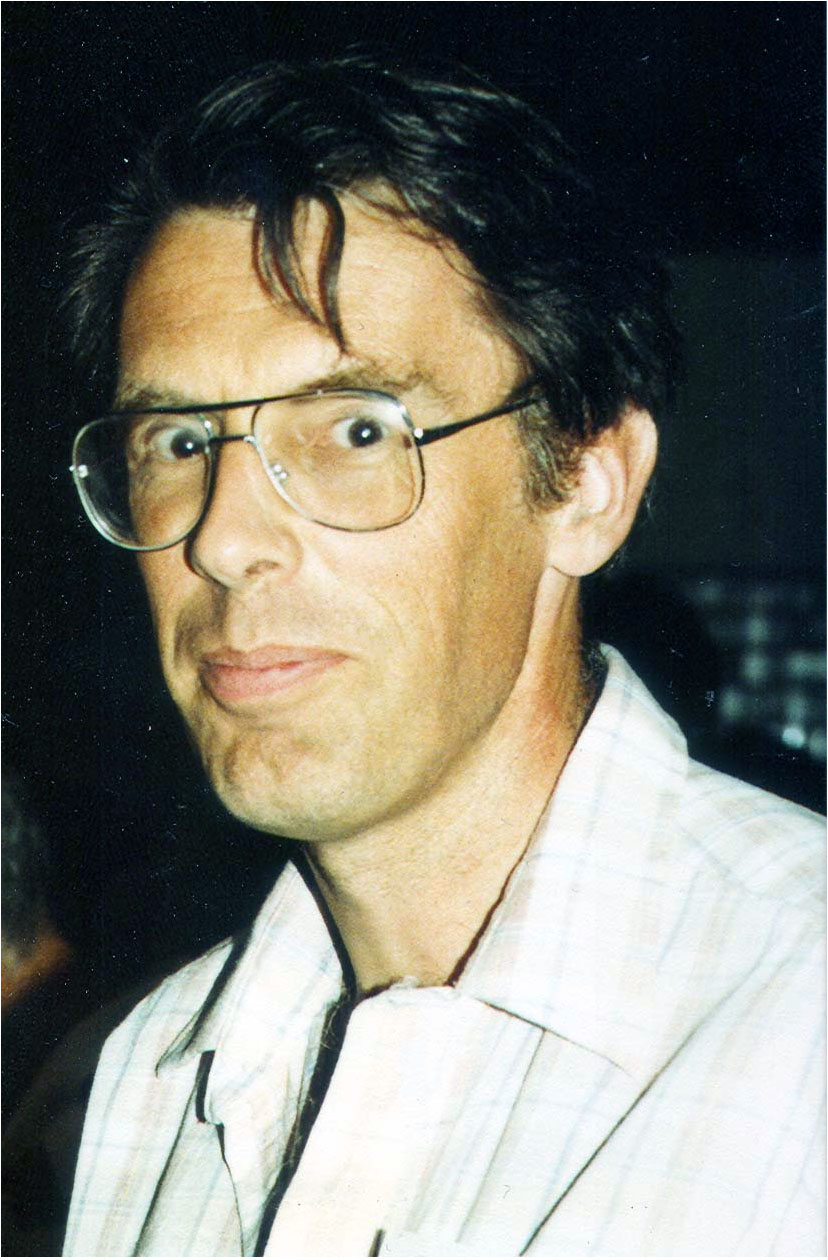
\includegraphics[height=2.5cm]{jehyoung.jpg}\hspace{0.1cm}\footnotemark};
		\end{tikzpicture}
		
		\footnotetext{\tiny\url{http://www.cs.cornell.edu/gries/banquets/symposium40/images/faculty/jehyoung.jpg}}
		
		\vspace{-0.4cm}
		\noindent MinimizeDFA($A$)
		
		\begin{enumerate}
		\item Compute all unreachable states
		\item Remove all unreachable states and their transitions
		\item Compute all inequivalent state pairs ($\not\sim_A$)
		\begin{algorithmic}[1]
			\Function{\CompDist}{$A$}
			\State $i \gets 0$
			\State $m(0) \gets \{ (p,q), (q,p)\ |\ p \in F, q \notin F \}$
			\Do
			\State $i \gets i + 1$
			\State $m(i) \gets \{ (p,q), (q,p)\ |\ (p,q) \notin \bigcup{m(\cdot)} \land$
			\State \hfill$\exists \sigma \in \Sigma \colon (\delta(p,\sigma), \delta(q,\sigma)) \in m(i-1) \}$
			\doWhile {$m(i) \neq \emptyset$}
			\State \Return $\bigcup{m(\cdot)}$
			\EndFunction
		\end{algorithmic}
		\item Merge all equivalent state pairs
		\end{enumerate}
		
		\note{gehe auch hier davon aus\\zur Erinnerung\\-\\}
		
		\note{wir init. eine Menge m(0) mit Zustandspaaren, von denen je genau ein Zustand akzeptierend ist\\-\\}
		
		\note{neue Menge m(i); Zustandspaare (p,q), (p,q) in keiner vorher ber. Menge, und Paar delta p sigma, delta q sigma ist in Vorgängermenge}
	\end{frame}

	
	\begin{frame}
		\frametitle{Problem definition}
		\framesubtitle{A sample DFA minimization task\ldots}
		{\raggedright\itshape \underline{Task:} Consider the below shown deterministic finite automaton $A$:}
		\begin{center}\resizebox{.75\linewidth}{!}{
				\begin{tikzpicture}[initial text={},scale=1., every node/.style={transform shape}]
				\tikzstyle{every state}=[minimum size=5mm, inner sep=0pt]
				
				\node[initial, state]  (0) at (0, 0)    {$0$};
				\node[state] 		   (1) at (6, 0)    {$1$};
				\node[state,accepting] (2) at (4,0)     {$2$};
				\node[state]           (3) at (2, -1.5) {$3$};
				\node[state,accepting] (4) at (4,-3)    {$4$};
				\node[state]           (5) at (4,-1.5)  {$5$};
				\node[state]           (6) at (2,0)     {$6$};
				
				\path[->]
				(0) edge node [above=-0.07cm]  {$a$}   (6)
				(0) edge [bend left] node [above=-0.07cm]  {$b$}   (2)
				
				(1) edge node [above=-0.07cm]  {$a$}   (2)
				(1) edge node [below right=-0.15cm]  {$b$}   (4)
				
				(2) edge [bend left] node [above=-0.07cm]  {$a$}   (1)
				(2) edge node [below right=-0.15cm]  {$b$}   (3)
				
				(3) edge node [left=-0.07cm]  {$a$}   (6)
				(3) edge node [above right=-0.15cm]  {$b$}   (4)
				
				(4) edge [bend right] node [below right=-0.15cm]  {$a$}   (1)
				(4) edge [bend left] node [below left=-0.15cm]  {$b$}   (0)
				
				(5) edge node [below right=-0.15cm]  {$a$}   (1)
				(5) edge node [left=-0.07cm]  {$b$}   (4)
				
				(6) edge [bend right] node [below=-0.07cm]  {$a$}   (1)
				(6) edge node [above=-0.07cm]  {$b$}   (2)
				;
				\end{tikzpicture}
		}\end{center}
		{\itshape Apply the minimization algorithm and illustrate for each state pair of $A$ during which \CompDist-iteration it was marked. Draw the resulting automaton.}
		
		\note{auf dieser Folie... Bsp DFA-Minimierungsaufgabe}
	\end{frame}


	\begin{frame}
		\frametitle{Problem definition}
		\framesubtitle{\ldots and its solution}
	
		{\raggedright\itshape \underline{Solution:}\newline
			Step 1: Detect and eliminate unreachable states.
			\begin{tabbing}
				\qquad\textnormal{State $5$ is unreachable.}
			\end{tabbing}
			Step 2: Apply \CompDist\ to $A$ and merge equivalent state pairs:\par
		}
		\begin{columns}
		\begin{column}{.4\textwidth}
			\vspace{0.5cm}
			\qquad
			\begin{tabular}{c|c|c|c|c|c|c}
				& 0  & 1  & 2  & 3  & 4  & 6  \\\hline
				0 & \x & 1  & 0  &    & 0  & 2  \\\hline
				1 & \x & \x & 0  & 1  & 0  & 1  \\\hline
				2 & \x & \x & \x & 0  &    & 0  \\\hline
				3 & \x & \x & \x & \x & 0  & 2  \\\hline
				4 & \x & \x & \x & \x & \x & 0  \\\hline
				6 & \x & \x & \x & \x & \x & \x \\
			\end{tabular}
		\end{column}
		\begin{column}{.5\textwidth}\centering\resizebox{1.\linewidth}{!}{
			\begin{tikzpicture}[initial text={},scale=1., every node/.style={transform shape}]
			\tikzstyle{every state}=[minimum size=5mm, inner sep=0pt]
			
			\node[initial, state]  (03) at (0, 0)   {$03$};
			\node[state] 		   (1) at (6, 0)   {$1$};
			\node[state,accepting] (24) at (4,0)    {$24$};
			\node[state]           (6) at (2,0)    {$6$};
			
			\path[->]
			(03) edge node [above=-0.07cm]  {$a$}   (6)
			(03) edge [bend left] node [above=-0.07cm]  {$b$}   (24)
			
			(1) edge node [above=-0.13cm]  {$a,b$}   (24)
			
			(24) edge [bend left=50] node [above=-0.07cm]  {$a$}   (1)
			(24) edge [bend right=50] node [above=-0.07cm]  {$b$}   (03)
			
			(6) edge [bend right] node [below=-0.07cm]  {$a$}   (1)
			(6) edge node [above=-0.07cm]  {$b$}   (24)
			;
			\end{tikzpicture}
		}\end{column}
		\end{columns}
		\note{Lsg, die dadurch zustandekommt, dass man Hop. Min.alg. anwendet}
	\end{frame}

	\begin{frame}
		\frametitle{Problem Definition and Approach}
		
		DFAMinimization\vspace{0.1cm}
		
		\qquad$\underline{Given:}$ \emph{A DFA $A_{task}$.}
		
		\qquad$\underline{Task:}$ \emph{Compute $A_{sol} = \MinAlg(A_{task})$.}
		
		\vspace{0.2cm}
		Main question: How to generate instances of DFAMinimization?\pause
		
		\vspace{0.2cm}
		Idea: First generate $A_{sol}$, then add equivalent, then unreachable states.
		
		\vspace{0.4cm}
		\begin{tikzpicture}[initial text={}, every node/.style={transform shape}]
		
		\node[draw,style={rounded corners}] (p) at (0,0) {Parameters}; % $\nSO, \kAL, \nF, d, p_{sol}, p_{task}, \nEQ,\nUN, c$
		
		\node[draw] (1) at (0,-2) {
			\begin{minipage}{\linewidth}
			Generate DFA Minimization Problem
			
			\begin{itemize}
				\item Generate Minimal DFA
				
				\qquad (using a rejection algorithm and randomization/enumeration)
				
				\item Extend Minimal DFA
				\begin{itemize}
					\item Add Equivalent States
					\item Add Unreachable States
				\end{itemize}
			\end{itemize}
			
			\end{minipage}
		};
	
		\node[draw,style={rounded corners}] (o) at (0,-4) {$A_{task}$};
		
		\path[->]
		(p) edge (1)
		(1) edge (o)
		;
		\end{tikzpicture}
		\note{Eine Min.aufgabe können wir wie folgt formalisieren\\-\\}
		\note{in Anlehnung an H.Min.alg.\\-\\}
		\note{in meiner Arbeit... Reihe an Parametern, mit denen man versch. Eig. des gen. Problems beeinfl. kann\\-\\}
		\note{Trial-and-Error-Methode}
	\end{frame}
	
	
	\section{Generating Minimal DFAs}
	
	\begin{frame}
		\frametitle{Outline}
		\tableofcontents[currentsection] % [pausesections]
	\end{frame}
	
	\begin{frame}
		\frametitle{Generating Minimal DFAs}
		\framesubtitle{Rejection Algorithm}
		Approach: Generate test DFAs until they match the demanded properties.
		
		\vspace{0.2cm}
		\begin{algorithmic}[1]
			\Function{GenNewMinDFA\ }{$\nSO, \kAL, \nF, d, p$}
			
			\vspace{0.2cm}
			
			\State $l \gets$ all DFAs in DB$_{found}$ matching $\nSO, \kAL, \nF$
			
			\vspace{0.2cm}
			
			\While {True}
			
				\vspace{0.2cm}
				
				\State generate DFA $A_{test}$ with $|Q|, |\Sigma|, |F|$ matching $\nSO, \kAL, \nF$
	
				\vspace{0.2cm}
				
				\If {$A_{test}$ not minimal \textbf{or} $d \neq \mmD(A_{test})$}
					\State \textbf{continue}
				\EndIf
				
				\If {$p = 1$ \textbf{and} $A_{test}$ is not planar}
					\State \textbf{continue}
				\EndIf
				
				\If {$A_{test}$ is isomorph to any DFA in $l$}
					\State \textbf{continue}
				\EndIf
				
				\vspace{0.2cm}
				
				\State save $A_{test}$ and its respective properties in DB$_{found}$
				\State\Return $A_{test}$
			
			\EndWhile
			\EndFunction
		\end{algorithmic}
	
		\begin{tikzpicture}[remember picture,overlay]
		\node[xshift=-1.5cm,yshift=-6.25cm] at (current page.north east) {
\includegraphics[height=1.75cm]{rejection.jpg}\hspace{0.1cm}\footnotemark};
		\end{tikzpicture}
		
		\footnotetext{\tiny\url{https://moviewriternyu.files.wordpress.com/2015/10/rejection.jpg}}
		
		\note[item]{while-Schleife}
		\note[item]{test DFA generieren, für die schon drei Parameter garantiert stimmen, nämlich im Enzelnen}
		\note[item]{restl. Eig. werden in z. 5-10, bsp. 5 minimalität}
		\note[item]{wenn es Fragen zu den and. get. Eig. gibt, dann kann ich hier gerne im Anschluss genauere Erläuterungen geben}
		\note[item]{Hier möchte.. nur auf test DFA Generierung in z.4 näher eingehen}
	\end{frame}

	\begin{frame}
		\frametitle{Generating Minimal DFAs}
		\framesubtitle{Test DFA Generation}
		We will restrict ourselves to $Q = [0,\nSO-1],\ \Sigma = [0,\kAL-1],\ s = 0$.\\ $ $\\\pause
		
		\noindent Generation...
		\begin{enumerate}
			\item[(a)] by randomization:
			\begin{align*}
			F &= random\_subset(Q)\\
			\delta(q, \sigma) &= choose\_one(Q) \qquad\qquad \forall q\in Q, \sigma\in\Sigma
			\end{align*}\pause
			
			\item[(b)] by enumeration: An \emph{enumeration state} $s_{\nSO, \kAL, \nF} = (F_F,F_\delta)$ has the following semantics:
			\begin{align*}
			F_F[i] = 1 &\Leftrightarrow_{def} i \in F\\
			F_\delta[i * \kAL + j] = q &\Leftrightarrow_{def} \delta(i, j) = q
			\end{align*}
			Example state: $s_{4, 2, 2} = (0110)_2\ \ (10\ 13\ 22\ 03)_4$
		\end{enumerate}
		\note<1>{Im Rahmen dieser Arbeit\\}
		\note<2>{Ich werde hier zwei Methoden zur Gen vorstellen. Die Gen. per Randomisierung funkt. hier wie folgt\\-\\}
		\note<2>{Für die Tr.fkt. wird für jede Komb. eines Zustands und eines Symbols ein zufälliger Zustand ausgewählt\\}
		\note<3>{verwalten wir für eine gegebene Enumeration einen\\-\\}
		\note<3>{parametrisiert mit\\-\\}
		\note<3>{wenn i nicht akz., dann FF[i] = 0; für alle Zustände definiert\\-\\}
		\note<3>{2. Feld speichert für alle Komb. eines Zustands und eines Symbols zu welchem Zustand man gelangt\\-\\Unten angedeutet; Felder als Zahlen interpretieren; durch gewisse Inkrementierungsfkt. von einem DFA zum nächsten gelangen; nicht weiter ausführen}
	\end{frame}

%	\begin{frame}
%		\frametitle{Generating Minimal DFAs}
%		\framesubtitle{Incrementing Enumeration States}
%		
%		\gregor{Short demo how the associated DFA changes, when an enumeration state is incremented}
%	
%	\end{frame}
	
	\section{Extending Minimal DFAs}
	
	\begin{frame}
		\frametitle{Outline}
		\tableofcontents[currentsection] % [pausesections]
		
		\note{Kapitel der Lös.DFA Gen. abgeschlossen; widmen uns Erweiterung dieser DFAs hin zu Aufgaben-DFAs\\-\\}
		
		\note{Beschäftigung zunächst, gemäß vorhin vorg. Reihenfolge, mit Hinz. äqu. Z.}
	\end{frame}
	
	\begin{frame}
	\frametitle{Extending Minimal DFAs}
	\framesubtitle{Adding Equivalent States (1)}
	
	We now want to add states $r_1,\ldots,r_\nEQ$ to the solution DFA, such that every $r_i$ is equivalent to a state $e$ in the solution DFA:
	\[
	\forall i \in [1,\nEQ] \colon\ \exists e \in Q_{sol}\colon\ r_i \sim_A e
	\]
	Whenever we add a state $r_i$, we will first choose an $e\in Q_{sol}$, then we add the transitions of $r_i$.\pause
	\begin{example}\centering
	\begin{tikzpicture}[initial text={}]
	\tikzstyle{every state}=[minimum size=5mm, inner sep=0pt]
	
	\node[state, initial]  (0) at (0, 0)   {$0$};
	
	\node [fit=(0),draw,rounded corners, dashed] {};
	
	\node[state]  (1) at (2, 0)   {$1$};
	\uncover<2>{\node[state] (2) at (2, -1.5) {$2$};}
	\uncover<3-4>{\node[state,fill=SeaGreen] (2) at (2, -1.5) {$e$};}
	\node         (2p) at (2, -2.4) {};
	\uncover<4>{\node[state,fill=SeaGreen] (ri) at (2, -3) {$r_i$};}
	
	
	\uncover<2-3>{\node[fit=(1)(2)(2p),draw,rounded corners,dashed] {};}
	\uncover<4>{\node[fit=(1)(2)(2p)(ri),draw,rounded corners,dashed] {};}
	
	\node[state,accepting]  (3) at (4, 0)   {$3$};
	\node[state,accepting]  (4) at (4, -1.5)   {$4$};
	
	\node [fit=(3)(4),draw,rounded corners, dashed] {};
	
	\path[->]
	([yshift=0.05cm]0.east) edge node [above] {$a$} ([yshift=0.05cm]1.west)
	([yshift=-0.05cm]0.east) edge node [below] {$b$} ([yshift=-0.05cm]1.west)
	
	(1) edge node [above] {$a$} (3)
	(1) edge node [left] {$b$} (2)
	
	(2) edge node [above] {$a$} (4)
	(2) edge [loop below] node [below] {$b$} (2)
	;
	\end{tikzpicture}
	\end{example}
\note<1>{Sei nE die gewünschte Anzahl an paarweise versch. äqu. Zustandspaaren.\\-\\}
\note<1>{In diesem Verfahren werden die rI einzeln nacheinander hinzugefügt}
\note<2-4>{im Bsp könnten wir zunächst Zst. 2 als orig. aussuchen, und dann rI gedanklich zu dessen Äqu. hinzufügen\\-\\}
\note<2-4>{dann würden wir jetzt die Tr. hinzufügen, dabei beginnen wir mit den ausgehenden Tr.}
\end{frame}

\begin{frame}
	\frametitle{Extending Minimal DFAs}
	\framesubtitle{Adding Equivalent States (2) - Outgoing Transitions}
	
	Observation:
	\[r_i \sim_A e\ \Longrightarrow\ \forall \sigma \in \Sigma \colon [\delta(r_i, \sigma)]_{\sim_A} = [\delta(e, \sigma)]_{\sim_A}\]
	
	Consequently:
	\vspace{0.3cm}
	\begin{itemize}
		\item[R1:] For each symbol $\sigma \in \Sigma$ choose exactly one state $q\in[\delta(e, \sigma)]_{\sim_A}$ and set $\delta(r_i, \sigma) = q$.
	\end{itemize}
	\vspace{0.3cm}\pause

	\begin{example}\centering
	\begin{tikzpicture}[initial text={}]
	\tikzstyle{every state}=[minimum size=5mm, inner sep=0pt]
	
	\node[state, initial]  (0) at (0, 0)   {$0$};
	
	\node [fit=(0),draw,rounded corners, dashed] {};
	
	\node[state]  (1) at (2, 0)   {$1$};
	\node         (2p) at (2, -2.4) {};
	\node[state] (2) at (2, -1.5) {$e$};
	\node[state] (ri) at (2, -3) {$r_i$};
	
	\node[state,accepting]  (3) at (4, 0)   {$3$};
	\node[state,accepting]  (4) at (4, -1.5)   {$4$};
	
	\path[->]
	([yshift=0.05cm]0.east) edge node [above] {$a$} ([yshift=0.05cm]1.west)
	([yshift=-0.05cm]0.east) edge node [below] {$b$} ([yshift=-0.05cm]1.west)
	
	(1) edge node [above] {$a$} (3)
	(1) edge node [left] {$b$} (2)
	;
	
	\uncover<1>{
		\node [fit=(3)(4),draw,rounded corners, dashed] {};
		\node[fit=(1)(2)(2p)(ri),draw,rounded corners,dashed] {};
		\path[->]
		(2) edge node [above] {$a$} (4)
		(2) edge [loop below] node [below] {$b$} (2)
		;
	}
	
	\uncover<2>{
		\node [fit=(3)(4),draw,rounded corners, dashed, color=Blue, line width=1.5pt] {};
		\node[fit=(1)(2)(2p)(ri),draw,rounded corners,dashed] {};
		\path[->]
		(2) edge[color=Blue,line width=1.5pt] node [above] {$a$} (4)
		(2) edge [loop below] node [below] {$b$} (2)
		;
	}
	
	\uncover<3>{
		\node [fit=(3)(4),draw,rounded corners, dashed, color=Blue, line width=1.5pt] {};
		\node[fit=(1)(2)(2p)(ri),draw,rounded corners,dashed] {};
		\path[->]
		(2) edge[color=Blue,line width=1.5pt] node [above] {$a$} (4)
		(2) edge [loop below] node [below] {$b$} (2)
		
		(ri) edge[color=Red,line width=1.5pt] node[below right] {$a$} (4)
		;
	}

	\uncover<4>{
		\node [fit=(3)(4),draw,rounded corners, dashed] {};
		\node[fit=(1)(2)(2p)(ri),draw,rounded corners,dashed, color=Blue, line width=1.5pt] {};
		\path[->]
		(2) edge node [above] {$a$} (4)
		(2) edge[color=Blue,line width=1.5pt] [loop below] node [below] {$b$} (2)
		
		(ri) edge node[below right] {$a$} (4)
		;
	}

	\uncover<5>{
		\node [fit=(3)(4),draw,rounded corners, dashed] {};
		\node[fit=(1)(2)(2p)(ri),draw,rounded corners,dashed, color=Blue, line width=1.5pt] {};
		\path[->]
		(2) edge node [above] {$a$} (4)
		(2) edge[color=Blue,line width=1.5pt] [loop below] node [below] {$b$} (2)
		
		(ri) edge[bend left=1.5cm, color=Red,line width=1.5pt] node[left] {$b$} (1)
		(ri) edge node[below right] {$a$} (4)
		;
	}
	\end{tikzpicture}
	\end{example}
	\note{..dann sind folglich auch diejenigen Zust. äqu., wenn wir ein bel. Symbol von rI und e aus lesen\\-\\}
	\note{und setze diesen Zustand als Endzustand für delta(rI, sigma)\\-\\}
	\note{So konnten wir mit dieser Regel erreichen, dass jede Transition von rI in dieselbe Äqu.kl. führt, die wir err. würden, wenn wir der korresp. Tr. von e folgten}
\end{frame}

\begin{frame}
	\frametitle{Extending Minimal DFAs}
	\framesubtitle{Adding Equivalent States (3) - Ingoing Transitions}
	Let $q$ be a state s.t.\ $\delta(q,\sigma)=p$ and we want $\delta(q,\sigma)=r_i$.
	\begin{itemize}
		\item[] $q$ must remain in its equivalence class
		
		\item[$\Rightarrow$] $p$ must be in $[r_i]_{\sim_A} = [e]_{\sim_A}$
		
		\item[$\Rightarrow$] $q$ has to have a transition to some state in $[r_i]_{\sim_A} = [e]_{\sim_A}$\pause
	\end{itemize}

	Observation: Since $r_i$ must be reachable, we require that there is at least one such transition for which $q \neq r_i$ is true.\pause
	
	\vspace{0.2cm}
	Furthermore, we see that $p$ must have at least $2$ \emph{ingoing elements}.
	\[
	in(q) = |d^-(q)| + \begin{cases}
	1 & \text{if } s = q\\
	0 & \text{else}
	\end{cases}
	\]\pause
	\begin{itemize}
		\item[R2:] Choose at least one $((q, \sigma), p) \in \delta$ with $[p] = [e]$ and $in(p) \geq 2$. For at least one chosen transition  $q\neq r_i$ must be true. Remove each $((q, \sigma), p)$ from $\delta$ and add $((q, \sigma), r_i)$.
	\end{itemize}
	\note<2>{bug in thesis and program, erst nach Abgabe gefunden, entsprechend dort falsch geschrieben u. programmiert\\-\\}
	\note<1>{wir müssen Tr. klauen, weil es keine Tr. mit 'losen' Enden gibt- arbeiten mit kompletten DFAs}
	\note<3>{im Wesentlichen: p muss freie eingehende Tr. haben}
\end{frame}

\begin{frame}
\frametitle{Extending Minimal DFAs}
\framesubtitle{Adding Equivalent States (3) - Ingoing Transitions}

\begin{itemize}
	\item[R2:] Choose at least one $((q, \sigma), p) \in \delta$ with $[p] = [e]$ and $in(p) \geq 2$. For at least one chosen transition  $q\neq r_i$ must be true. Remove each $((q, \sigma), p)$ from $\delta$ and add $((q, \sigma), r_i)$.
\end{itemize}

	\begin{example}\centering
	\begin{tikzpicture}[initial text={}]
	\tikzstyle{every state}=[minimum size=5mm, inner sep=0pt]
	
	\node[state, initial]  (0) at (0, 0)   {$0$};
	
	\node [fit=(0),draw,rounded corners, dashed] {};
	
	\node[state]  (1) at (2, 0)   {$1$};
	\node         (2p) at (2, -2.4) {};
	\node[state] (2) at (2, -1.5) {$e$};
	\node[state] (ri) at (2, -3) {$r_i$};
	
	\node[fit=(1)(2)(2p)(ri),draw,rounded corners,dashed] {};
	
	\node[state,accepting]  (3) at (4, 0)   {$3$};
	\node[state,accepting]  (4) at (4, -1.5)   {$4$};
	
	\node [fit=(3)(4),draw,rounded corners, dashed] {};
	
	\path[->]
	([yshift=0.05cm]0.east) edge node [above] {$a$} ([yshift=0.05cm]1.west)
	
	(1) edge node [above] {$a$} (3)
	(1) edge node [left] {$b$} (2)
	
	(2) edge node [above] {$a$} (4)
	
	(ri) edge[bend left=1.5cm] node[left] {$b$} (1)
	(ri) edge node[below right] {$a$} (4)
	;
	
	\uncover<1>{
		\path[->]
		([yshift=-0.05cm]0.east) edge[color=Blue, line width=1.5pt] node [below] {$b$} ([yshift=-0.05cm]1.west)
		(2) edge [loop below, color=Blue, line width=1.5pt] node [below] {$b$} (2)
		;
	}
	
	\uncover<2>{
		\path[->]
		([yshift=-0.05cm]0.east) edge[color=Blue, line width=1.5pt] node [below] {$b$} ([yshift=-0.05cm]1.west)
		(2) edge[color=Red, line width=1.5pt] node[left] {$b$} (ri)
		;
	}

	\uncover<3>{
		\path[->]
		(0) edge[bend right=1.5cm, color=Red, line width=1.5pt] node[left] {$b$} (ri)
		(2) edge[color=Red, line width=1.5pt] node[left] {$b$} (ri)
		;
	}
	\end{tikzpicture}
\end{example}

\end{frame}

	\begin{frame}
		\frametitle{Extending Minimal DFAs}
		\framesubtitle{Adding Unreachable States}
	
		Reminder: We say a state $q$ is \emph{unreachable}, iff there is no word $w \in \Sigma^*$ such that $\delta^*(s, w) = q$.
		\vspace{0.3cm}
	
		\begin{algorithmic}[1]
			\Function{AddUnrStates\ }{$A, \nUN, c$}
			\State $U \gets \emptyset$
			\vspace{0.2cm}
			
			\For {$\nUN$ \textbf{times}}
				\vspace{0.2cm}
				
				\State let $q$ be the new state
				\vspace{0.2cm}
				
				\State steal ingoing tr.\ from a random subset of $U\times\Sigma$
				\State add outgoing tr.\ to $|\Sigma|$ random states
				\vspace{0.2cm}
				
				\State add $q$ to $U$
			\EndFor
			\vspace{0.2cm}
			
			\State \Return $A$
			\EndFunction
		\end{algorithmic}
%	
%		\begin{tikzpicture}[remember picture,overlay]
%		\node[xshift=-1.5cm,yshift=-7.5cm] at (current page.north east) {
\includegraphics[height=1.75cm]{Fix-err-address-unreachable.jpg}};
%		\end{tikzpicture}
	
	\end{frame}

	\section{Live Demonstration and Conclusion}
	
	\begin{frame}
		\frametitle{Outline}
		\tableofcontents[currentsection] % [pausesections]
	\end{frame}

	\begin{frame}
		\frametitle{Live Demonstration}
		\centering\vspace{1cm}
		\hspace{0.2cm}
\includegraphics[width=0.95\linewidth]{loading-100.png}\hspace{0.1cm}\footnotemark
		
		\footnotetext{\tiny\url{https://sagamer.co.za/wp-content/uploads/2015/03/loading-please-wait.png}}
	\end{frame}
	
%	\begin{frame}
%		\frametitle{Live Demonstration}
%		\framesubtitle{Program Architecture}
%		\begin{tikzpicture}[initial text={}, every node/.style={transform shape}]
%		
%		\node[draw] (main) at (0,0) {main.py};
%		
%		\node[draw,style={rounded corners}] (log) at (3,0) {log.py};
%		
%		\node[draw] (build) at (-3,-1.5) {build.py};
%		\node[draw] (extend) at (0,-1.5) {extend.py};
%		\node[draw] (output) at (3,-1.5) {output.py};
%		
%		\node[draw] (dbdfa) at (-4,-3) {db\_dfa.py};
%		\node[draw] (dbenum) at (-2,-3) {db\_enum.py};
%		
%		\node[draw] (iso) at (-3, -4.5) {isomorphy.py};
%		\node[draw] (min) at (0, -4.5) {minimization.py};
%		\node[draw] (plan) at (3, -4.5) {planarity.py};
%		
%		\node[draw, fit=(iso)(plan)] (iso) at (0, -5.3) {dfa.py};
%		
%		\path[->]
%			(main) edge (log)
%			
%			(main) edge (build)
%			(main) edge (extend)
%			(main) edge (output)
%			
%			(build) edge (dbdfa)
%			(build) edge (dbenum)
%		;
%		\end{tikzpicture}
%	\end{frame}

%	\begin{frame}
%		\frametitle{Live Demonstration}
%		\framesubtitle{Command-Line Options}
%		
%		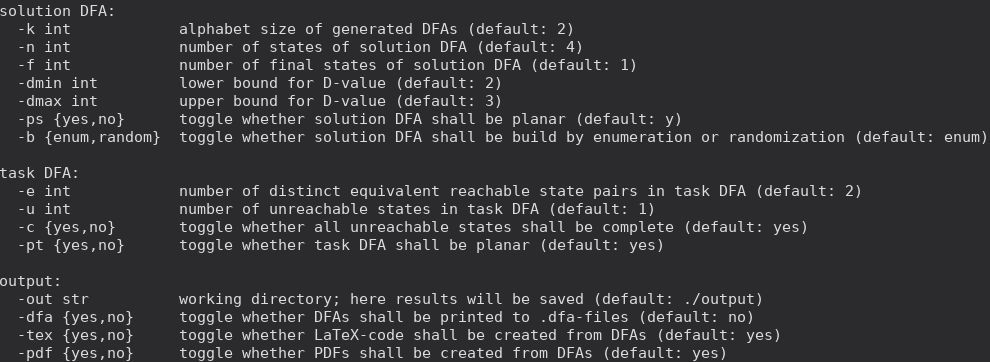
\includegraphics[width=\linewidth]{options.jpg}
%		\gregor{Replace}
%	
%	\end{frame}
	
%	\section{Conclusion}
	
%	\begin{frame}
%		\frametitle{Outline}
%		\tableofcontents[currentsection] % [pausesections]
%	\end{frame}

	\begin{frame}
		\frametitle{Conclusion}
		
		This presentation has\ldots
		\begin{itemize}
			\item introduced the problem of DFA Minimization Problem Generation
			\item given an overview over a possible solution
			\item shown that the theoretic results might be useful in praxis
		\end{itemize}\pause
		Lookout:
		\begin{itemize}
			\item more parameters, ranged parameters
			
			The \emph{degree} of a state $q$ is defined as $deg(q) = |d^-(q)| + |d^+(q)|$.
			
			$\Rightarrow$ capping the max.\ degree?
			
			\item investigate planarity and drawing algorithms
			\item complexity analysis
		\end{itemize}\pause
		\vspace{0.4cm}
		\begin{center}
			\uncover<3-4>{Thanks for listening}\uncover<3>{!}\uncover<4>{even longer!}
		\end{center}
	
	\end{frame}

	\begin{frame}
		\frametitle{Bonus-Slide}
		\framesubtitle{$\mmD$-Proof}
		
		\begin{definition} \label{ch:4:def-dist-word}
			We will call a word $w$ \emph{distinguishing word of $p,q$}, iff
			\[
				\delta^*(p,w) \in F \Leftrightarrow \delta^*(q,w) \notin F		
			\]
%				\item \emph{finishing word of $q$}, iff $\delta^*(q, w) \in F$
		\end{definition}
		\vspace{-0.7cm}
		\begin{lemma}\label{ch:4:semantics-of-m(n)}
			Iff $(p,q)\in m(n)$, the shortest distinguishing word of $p,q$ has length $n$.
		\end{lemma}
	
		\begin{lemma}\label{ch:4:semantics-of-D(A)}
			If \CompDist\ has done $n$ iterations and terminated (so $\mmD(A) = n$), then the longest word $w$, that is a shortest distinguishing word for any state pair, has length $\mmD(A)-1$.
		\end{lemma}
	
		\begin{theorem}\label{ch:4:th-D}
			Given two DFAs $A$, $A'$. If both are accessible and $L(A) = L(A')$, then \CompDist\ runs with the same number of iterations on them: $\mmD(A) = \mmD(A')$.
		\end{theorem}
	
	\end{frame}
%
%	\begin{frame}
%		\frametitle{Bonus-Slides}
%		\framesubtitle{$\mmD$-Proof}
%		
%			\begin{itemize}
%				\item [] $L(A) = L(A') \Rightarrow \forall w \in \Sigma^*\colon \delta^*(s, w) \in F \Leftrightarrow \delta'^*(s', w) \in F'$\pause
%				
%				We extend this to a statement that includes any state visited on the way to $F$ resp.\ $F'$.
%				\vspace{0.2cm}
%				
%				
%				\item[$\Rightarrow$] $\forall u \in \Sigma^*\colon \exists q,q' \in Q\colon$
%				
%				\qquad $\delta^*(s, u) = q \land \delta'^*(s', u) = q' \land$
%				
%				\qquad $f(q) = f(q')$\pause
%				
%				Since all states in $A$/$A'$ are reachable:
%				\vspace{0.2cm}
%				
%				
%				\item [$\Rightarrow$] $\forall q \in Q\colon \exists q' \in Q'\colon f(q) = f(q')$ $\land$ 
%				
%				$\forall q' \in Q'\colon \exists q \in Q\colon f(q) = f(q')$
%				
%				\item[$\Rightarrow$] $\{\ f(q)\ |\ q \in Q\ \} = \{\ f(q')\ |\ q' \in Q'\ \}$\pause
%				
%				\item[$\Rightarrow$] There cannot be a distinguishing word in one of $A$/$A'$ that is not distinguishing word in the other DFA.
%				\vspace{0.2cm}
%				
%				\item[$\Rightarrow$] Both DFAs have the same shortest distinguishing words and thus too the same longest shortest distinguishing word.
%				
%				\item[$\Rightarrow$] If $\mmD(A) \neq \mmD(A')$, then one DFA would have a longer longest shortest distinguishing word $\Rightarrow \mmD(A) = \mmD(A')$
%			\end{itemize}
%	\end{frame}
%
%	\begin{frame}
%	\frametitle{Bonus-Slides}
%	\framesubtitle{Ideas for further Works}
%	\end{frame}
%
%	\begin{frame}
%	\frametitle{Bonus-Slides}
%	\framesubtitle{Small Project-History}
%	\end{frame}

\end{document}

